\documentclass[aspectratio=169,usenames,dvipsnames]{beamer}

\mode<presentation>{
  \usetheme{default}
  \usecolortheme{default}
  \usefonttheme{default}
}

% ------------------------------------------------
% Colors
% ------------------------------------------------
\usepackage{xcolor}
\definecolor{purple}{HTML}{695693}
\definecolor{navy}{HTML}{567293}
\definecolor{ruby}{HTML}{9a2515}
\definecolor{alice}{HTML}{107895}
\definecolor{daisy}{HTML}{EBC944}
\definecolor{coral}{HTML}{F26D21}
\definecolor{kelly}{HTML}{829356}
\definecolor{cranberry}{HTML}{E64173}
\definecolor{jet}{HTML}{131516}
\definecolor{asher}{HTML}{555F61}
\definecolor{slate}{HTML}{314F4F}
\definecolor{accent}{HTML}{107895}
\definecolor{accent2}{HTML}{9a2515}

\definecolor{blue1}{RGB}{27,  98, 168}
\definecolor{blue2}{RGB}{67, 135, 195}
\definecolor{blue3}{RGB}{114,169, 211}
\definecolor{blue4}{RGB}{169,206, 227}
\definecolor{redUT}{RGB}{215, 48,  39}

% ------------------------------------------------
% Fonts & math
% ------------------------------------------------
\usepackage[T1]{fontenc}
\usepackage{amsmath, amssymb}
\usepackage{setspace}
\usepackage{bbm}

% ------------------------------------------------
% Tables / figures
% ------------------------------------------------
\usepackage{geometry}
\usepackage{float}
\usepackage{booktabs}
\usepackage{multirow}
\usepackage{graphicx}
\usepackage{subfigure}
\usepackage{array}
\usepackage{tabularx}
\usepackage{threeparttable}
\usepackage{makecell}
\newcolumntype{C}{>{\centering\arraybackslash}X}

% ------------------------------------------------
% TikZ
% ------------------------------------------------
\usepackage{tikz}
\usetikzlibrary{calc}
\usetikzlibrary{fit,shapes.misc}
\usetikzlibrary{tikzmark}
\usepackage{colortbl}

% ------------------------------------------------
% Misc
% ------------------------------------------------
\usepackage{comment}
\usepackage{caption}
\usepackage{color}

% ------------------------------------------------
% Bibliography
% ------------------------------------------------
\usepackage[round, authoryear]{natbib}
\bibliographystyle{chicago}

\newcommand{\smallcite}[1]{{\footnotesize\textcolor{Blue}{\citep{#1}}}}

% ------------------------------------------------
% Hyperref
% ------------------------------------------------
\usepackage{hyperref}
\hypersetup{
    colorlinks=true,
    citecolor=Blue,
    linkcolor=Blue,
    urlcolor=Blue
}

% ------------------------------------------------
% Beamer colors
% ------------------------------------------------
\setbeamertemplate{navigation symbols}{}
\setbeamercolor{frametitle}{fg=Blue}
\setbeamercolor{item projected}{fg=Blue}
\setbeamercolor{title}{fg=Blue}
\setbeamercolor{section in head/foot}{fg=Blue}
\setbeamercolor{subsection in head/foot}{fg=Blue}

% ------------------------------------------------
% Footline
% ------------------------------------------------
\setbeamertemplate{footline}{
  \leavevmode
  \hbox{
  \begin{beamercolorbox}[wd=.333333\paperwidth,ht=2.25ex,dp=1ex,center]{title in foot}
    \usebeamerfont{title in foot}\insertsection
  \end{beamercolorbox}
  \begin{beamercolorbox}[wd=.333333\paperwidth,ht=2.25ex,dp=1ex,center]{date in foot}
    \usebeamerfont{date in foot}\hspace*{2em}
  \end{beamercolorbox}
  \begin{beamercolorbox}[wd=.333333\paperwidth,ht=2.25ex,dp=1ex,right]{number in foot}
    \usebeamerfont{numb in foot}\insertframenumber{}/\inserttotalframenumber{}\hspace*{2em}
  \end{beamercolorbox}}
  \vskip1pt
}

% ------------------------------------------------
% Backup slides
% ------------------------------------------------
\newcommand{\backupbegin}{
   \newcounter{finalframe}
   \setcounter{finalframe}{\value{framenumber}}
}

\newcommand{\backupend}{
   \setcounter{framenumber}{\value{finalframe}}
}

% ------------------------------------------------
% Graphics
% ------------------------------------------------
\graphicspath{{figures/}}

% ------------------------------------------------
% TITLE
% ------------------------------------------------
% ------------------------------------------------
% TITLE
% ------------------------------------------------
\title[W]{\LARGE{Do Conditional Cash Transfer Programs Reduce Mortality?\\Ten-Year Evidence from Mexico}}

\author[]{%
  \texorpdfstring{%
    \begin{tabular}{c c c}
      Emma Aguila & William H.\ Dow & Felipe Menares$^{*}$ \\
      \textcolor{gray}{USC} & \textcolor{gray}{UC Berkeley} & \textcolor{gray}{Inter-American Development Bank} \\[4pt]
      Susan W.\ Parker & Jorge Peniche & Soomin Ryu \\
      \textcolor{gray}{University of Maryland} & \textcolor{gray}{USC} & \textcolor{gray}{University of Missouri} \\
    \end{tabular}
  }
  {Emma Aguila, William H. Dow, Felipe Menares, Susan W. Parker, Jorge Peniche, Soomin Ryu}
}

\date{November 2026}

% ------------------------------------------------
% DOCUMENT
% ------------------------------------------------
\begin{document}

\setlength{\abovedisplayskip}{3pt}
\setlength{\belowdisplayskip}{3pt}

{
\setbeamertemplate{footline}{}
\begin{frame}
  \titlepage
  \vfill
  {\tiny $^{*}$The opinions expressed in this paper are those of the authors and do not necessarily reflect the views of the Inter-American Development Bank, its Board of Directors, or the countries they represent, nor of INEGI.}
\end{frame}
}
\note{Hello everyone. Today I'm presenting joint work on whether Mexico's Progresa conditional cash transfer program reduced elderly mortality. Our paper asks whether a program primarily designed to invest in children's education and health produced meaningful mortality benefits for the elderly over a longer time horizon.}

%%%%%%%%%%%%%%%%%%%%%%%%%%%%%%%%%%%%%%%%
%%% MOTIVATION %%%
%%%%%%%%%%%%%%%%%%%%%%%%%%%%%%%%%%%%%%%%
\section{Background}

\begin{frame}{Motivation: Older adults are the fastest-growing population group}\label{motivation}
\vspace{2pt}
\small
\begin{itemize}
  \item[$\circ$] In LAC, ~10\% of the population is 65+ (2024), projected to reach double by 2050 \smallcite{UN2024WPP}; 1 in 5 older adults lives in multidimensional poverty \smallcite{CEPAL2024SocialPanorama}
  \item[$\circ$] Income support programs and health: evidence is mixed
    \begin{itemize}
      \item Some studies find important health benefits \smallcite{Case2004PerspectivesAging, Aguila2015PNAS}, others find no effects \smallcite{LloydSherlockAgrawal2014JDS}, and some identify unintended adverse consequences \smallcite{FernaldGertlerHou2008JN}
    \end{itemize}
  \vspace{4pt}
  \item[$\circ$] Most existing evidence focuses on \textbf{short-run} rather than long-run \textbf{mortality} effects
  \vspace{4pt}
  \item[$\circ$] CCTs have been widely studied for children, but \textbf{elderly} has been overlooked
    \begin{itemize}
      \item improved health-service utilization for elderly women \smallcite{BehrmanParker2013Demography}
      \item higher hypertension diagnosis, but no improvement in biomarkers \smallcite{aguila2024conditional}
      \item
      \textit{short-run} reductions in elderly mortality over first years \smallcite{BarhamRowberry2013JDE}
    \end{itemize}
  \vspace{4pt}
  \item[$\circ$] \textbf{Direct} pension programs for older adults show larger effects
    \begin{itemize}
      \item Mexico's \textit{70 y Más}: $-5.5\%$ elderly women mortality \smallcite{Menares2026JHR}
    \end{itemize}
\end{itemize}
\end{frame}

\note{The broader literature on income transfers and health yields mixed results. Some find benefits, others find none. Most evidence is short-run. For the elderly specifically, we know Progresa increased clinic visits but didn't improve blood pressure biomarkers. Barham and Rowberry provided the key short-run mortality finding. And we know that pension programs that transfer directly to the elderly show stronger effects.}

\begin{frame}{This Paper: Did \textit{earlier} exposure to \textit{Progresa} reduce older adult mortality?}\label{thispaper}
\vspace{0pt}
\small
\begin{itemize}
  \item[$\circ$] \textbf{Identification:} DiD across highly marginalized municipalities (1991--2006) with different early (1997--1999) enrollment but \textbf{similar coverage by 2005}
    \begin{itemize}
      \item Effect of $\approx$4--5 \textit{additional} years of exposure, not program vs.\ no program
    \end{itemize}
  \vspace{2pt}
  \item[$\circ$] \textbf{Main finding:} \textcolor{redUT}{No detectable reduction in older-adult mortality}
    \begin{itemize}
      \item Robust to weighting, functional form, SES trends, Seguro Popular; detects effects $\geq 4.1$ deaths/1,000
    \end{itemize}
  \vspace{2pt}
  \item[$\circ$] \textbf{Revisiting prior evidence:} Short-run estimates of \cite{BarhamRowberry2013JDE} are sensitive and depend on weighting and sample
    \begin{itemize}
      \item Population weights attenuate them by $\approx 50\%$; no clean post-1997 break in the event study
    \end{itemize}
  \vspace{2pt}
  \item[$\circ$] \textbf{Mechanisms (experimental data):} no effects on labor supply or health visits; limited changes in household composition
\end{itemize}
\end{frame}

\note{Our paper re-examines this question using sixteen years of vital statistics. Note what we estimate: municipalities end up with similar coverage by 2005, so we compare earlier versus later exposure — roughly four to five extra years — not Progresa versus no Progresa. The main finding is that earlier exposure did not detectably reduce older-adult mortality, and our design has the power to detect effects of the size previously reported. The earlier short-run estimate becomes much smaller once we weight by population and is sensitive to the sample. In the experimental data, we find no effects on labor supply or health visits and only limited changes in living arrangements.}

%%%%%%%%%%%%%%%%%%%%%%%%%%%%%%%%%%%%%%%%
%%% PROGRAM BACKGROUND %%%
%%%%%%%%%%%%%%%%%%%%%%%%%%%%%%%%%%%%%%%%
\section{Program}

\begin{frame}{Mexico's \textit{Progresa}: Launched 1997 in small rural localities}\label{progresa}
\footnotesize
\begin{itemize}
  \item[$\circ$]  Targeted poor households reaching $\frac{1}{4}$ and $\frac{2}{3}$ in localities $<$2,500 inhabitants
  %(locality marginality index and a household-level proxy means test)
  %\vspace{1pt}
  %\item[$\circ$] \textbf{Scale:} 6 million families covered (
  
  \vspace{1pt}

  \item[$\circ$] \textbf{Transfer:} Represented a $25\%$ income increase); paid to female household head
    \begin{itemize}
      \item \textit{Education grant:} households with children attending school ($\geq 85\%$ attendance)
      \item \textit{Food transfer:} flat rate to \textbf{every} eligible household, incl.\ older-adults-only households
    \end{itemize}
  \vspace{1pt}
  \item[$\circ$] \textbf{Health conditionality:} all members visit clinic; adults $17+$ (incl.\ elderly): \textbf{one annual visit only}
  \vspace{1pt}
  \item[$\circ$] \textbf{In 2006:} pension for adults $70+$ added --- sample ends in 2006 (results unchanged excluding 2006)
  \vspace{1pt}
  \item[$\circ$] \textbf{Elderly in eligible households:}
    \begin{itemize}
      \item $\approx 75\%$ of elderly lived in households with children under 15 \smallcite{BehrmanParker2013Demography}
      \item Mostly grandparents, not direct recipients $\to$ benefits only through household sharing or indirect pathways
    \end{itemize}
\end{itemize}
\end{frame}

\note{Progresa started in 1997 in small rural localities and rapidly scaled. Transfers went to the female head of household. The education grant went to households with school-age children, but a flat food transfer went to every eligible household, including households made up only of older adults. For adults over 17, including the elderly, the health conditionality was just one annual clinic visit, a very minimal requirement. The elderly in these households are typically grandparents who don't control program funds but might benefit through household resource sharing.}

\begin{frame}{Potential Channels to Elderly Mortality}\label{channels}
\footnotesize
\begin{columns}[T]
  \begin{column}{0.48\textwidth}
    \textbf{Theoretical channels}
    \vspace{4pt}
    \begin{enumerate}
      \item \textbf{Health conditionality} \\
        One annual clinic visit $\to$ early detection of diabetes, hypertension, infectious disease
      \vspace{3pt}
      \item \textbf{Income and nutrition} \\
        Improved nutrition and healthcare access for elderly members
      \vspace{3pt}
      \item \textbf{Labor supply} \\
        Less work $\to$ lower physical health risks (but possibly less social interaction)
      \vspace{3pt}
      \item \textbf{Living arrangements} \\
        More co-residence of family members $\to$ more informal caregiving for elderly
    \end{enumerate}
  \end{column}
  \begin{column}{0.48\textwidth}
    \textbf{Why each channel may not work}
    \vspace{4pt}
    \begin{itemize}
      \item[$\circ$] \textit{Health conditionality:} one annual visit is a minimal intervention; \cite{aguila2024conditional} find increased utilization but no improvement in blood pressure biomarkers
      \vspace{4pt}
      \item[$\circ$] \textit{Income:} transfers go to female head and are labeled for children's schooling; elderly members may not capture redistribution
      \vspace{4pt}
      \item[$\circ$] \textit{Labor supply / caregiving:} elderly are not the target; the physical-presence requirement for cash collection may \textit{increase} time demands on younger members \smallcite{BehrmanParker2013Demography}
    \end{itemize}
  \end{column}
\end{columns}
\end{frame}

\note{There are four plausible channels through which Progresa could affect elderly mortality: the health conditionality, income and nutrition, labor supply, and living arrangements. Each has a reason why it may not operate in practice. The clinic visit is minimal, the income is paid to mothers and labeled for children, and the elderly are not the target of the labor and caregiving responses. We test these channels with the experimental evaluation data and the ENIGH.}

%%%%%%%%%%%%%%%%%%%%%%%%%%%%%%%%%%%%%%%%
%%% DATA %%%
%%%%%%%%%%%%%%%%%%%%%%%%%%%%%%%%%%%%%%%%
\section{Data}

\begin{frame}{Data Sources}\label{data}
\footnotesize
\begin{itemize}
  \item \textbf{Mortality data} $\rightarrow$ primary outcome publicly available from INEGI
    \begin{itemize}
      \item Individual-level death registries from death certificates, 1991--2006 
      \item Includes cause of death, birth year, sex, municipality of residence
    \end{itemize}
  \vspace{1pt}
  \item \textbf{Population and household data} $\rightarrow$ mortality rate denominators
    \begin{itemize}
      \item Interpolated Census/counts 1990, 1995, 2000, 2005 by sex, age, municipality
      %geometrically 
    \end{itemize}
  \vspace{1pt}
  \item \textbf{\textit{Progresa} administrative data} $\rightarrow$ treatment variable
    \begin{itemize}
      \item Annual enrolled households by municipality over total households 
      %(linearly interpolated)
    \end{itemize}
  \vspace{1pt}
  \item \textbf{CONAPO Marginalization Index (1990)} $\rightarrow$ sample restriction
    \begin{itemize}
      \item Sample restricted to highly marginalized municipalities (grade 4 or 5)
    \end{itemize}
  \vspace{1pt}
  \item \textbf{\textit{Progresa} experimental surveys (ENCASEH 1997; ENCEL 1998--2000)} $\rightarrow$ mechanisms
    \begin{itemize}
      \item 506 treatment + 320 control localities; 18-month experimental window
      \item Labor supply, household composition, health visits for elderly $65+$ in eligible households
    \end{itemize}
  %\vspace{1pt}
  %\item \textbf{ENIGH (1992--2006)} $\rightarrow$ income and nutrition mechanisms (Household Survey)
\end{itemize}
\end{frame}

\note{We combine five data sources. The death registry covers every recorded death in Mexico from 1991 to 2006 — over three million records. The administrative enrollment data lets us measure Progresa intensity at the municipality level. The experimental evaluation data from 1997 to 2000 is the cleanest source for testing mechanisms. And the ENIGH household survey lets us look at income and nutrition.}

\begin{frame}{Sample and Trends}\label{trends}
\vspace{-3mm}
\begin{figure}
  \centering
  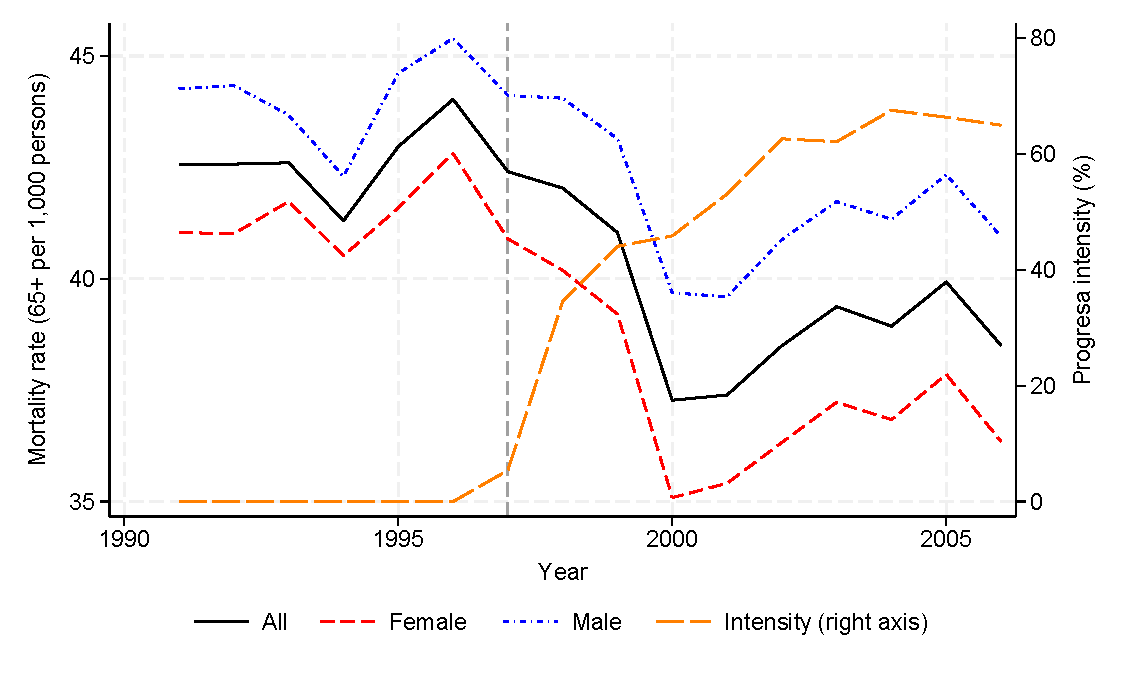
\includegraphics[width=0.89\textwidth, keepaspectratio]{Figure_1a_marg.pdf}
\end{figure}
\end{frame}

\note{This figure shows the key trends. The mortality rate for adults 65 and older in highly marginalized municipalities is on the left axis, and Progresa penetration is on the right. The vertical line marks 1997 when the program started. We can see that mortality was declining before the program, and enrollment grew rapidly after 1997. The identification challenge is separating the program's effect from the pre-existing trend.}

\begin{frame}{Geographic Distribution of Progresa Intensity}\label{maps}
\vspace{-2mm}
\begin{columns}
  \begin{column}{0.5\textwidth}
    \centering
    {(a) Intensity in 1999 (early phase)}\\
    \vspace{2pt}
    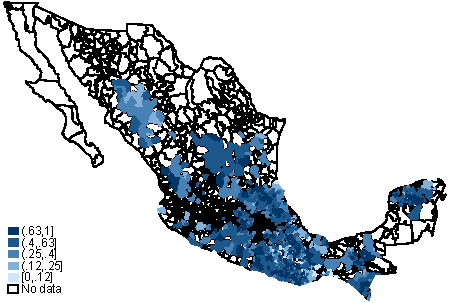
\includegraphics[width=\textwidth, keepaspectratio]{Figure_1b_inten1999.pdf}
  \end{column}
  \begin{column}{0.5\textwidth}
    \centering
    {(b) Intensity in 2005 (later phase)}\\
    \vspace{2pt}
    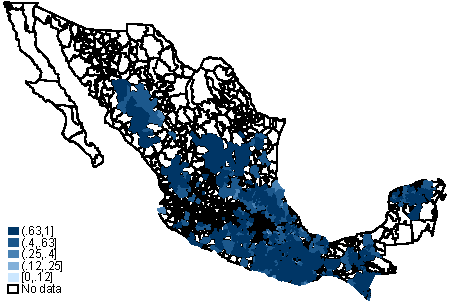
\includegraphics[width=\textwidth, keepaspectratio]{Figure_1c_inten2005.pdf}
  \end{column}
\end{columns}
% \vspace{2mm}
% {\footnotesize Municipality-level Progresa intensity (share of beneficiary households) among highly marginalized municipalities. Darker shading = higher intensity. Substantial variation across municipalities in both phases motivates the two-phase DiD design.}
\end{frame}

\note{These maps show the geographic distribution of Progresa intensity in 1999 and 2005. There is substantial variation across municipalities in both phases, and the geographic pattern shifts between early and late enrollment. This variation is what we exploit in the analysis.}

%%%%%%%%%%%%%%%%%%%%%%%%%%%%%%%%%%%%%%%%
%%% EMPIRICAL STRATEGY %%%
%%%%%%%%%%%%%%%%%%%%%%%%%%%%%%%%%%%%%%%%
\section{Empirical Strategy}

\begin{frame}{Empirical Strategy: Difference-in-Differences}\label{empirics}
\footnotesize
\begin{itemize}
  \item \textbf{Early phase:} $\textit{Intensity}_{m,1999}$ --- cumulative share of households enrolled by 1999 (mean 44\%)
  \item \textbf{Later phase:} $\textit{Intensity}_{m,2005}$ --- cumulative share enrolled by 2005 (mean 72\%), included as a \textbf{control}
  \item Common timing (1997) for all municipalities $\to$ no already-treated units used as controls (no forbidden comparisons)
\end{itemize}

\vspace{2pt}
\textbf{Baseline specification}
\vspace{-6pt}

\begin{equation*}
\text{MR}_{m,t}
= \beta_{0}\,\textit{Post}_{t} \times \textit{Intensity}_{m,1999}
+ \beta_{1}\,\textit{Post}_{t} \times \textit{Intensity}_{m,2005}
+ \delta_{m} + \gamma_{t} + \chi_{m,t} + \varepsilon_{m,t}
\end{equation*}

\vspace{-2pt}
\begin{itemize}
  \item $\text{MR}_{m,t}$: deaths per 1,000 aged $65+$; $\textit{Post}_{t} = 1$ for 1997--2006; $\delta_m$, $\gamma_t$: municipality and year FE
  \item $\chi_{m,t}$: Seguro Popular enrollment intensity (health insurance rollout from 2002)
  \item \textbf{Coefficient of interest}: $\beta_0$ --- effect of \textit{earlier} exposure ($\approx$4--5 extra years) among municipalities with \textbf{similar coverage by 2005}; ITT, not program vs.\ no program
  \item SE clustered by municipality; weighted by population 65+
  %$\beta_1$: control with no stand-alone interpretation (not reported); 
\end{itemize}

\end{frame}

\note{Our identification strategy compares municipalities that enrolled more households in the early phase of Progresa (1997-1999) with those that enrolled more later, holding cumulative coverage by 2005 fixed. Average enrollment goes from 44 percent in 1999 to 72 percent in 2005, so early enrollers get roughly four to five extra years of exposure. That is what beta zero measures: earlier exposure, not program versus no program. The 2005 intensity is a control and we do not interpret it. Because the post indicator turns on in 1997 for everyone, we avoid comparing already-treated to newly treated units. We control for Seguro Popular, Mexico's public health insurance that rolled out after 2002, and weight by the elderly population to avoid giving outsized influence to tiny, volatile municipalities.}

%%%%%%%%%%%%%%%%%%%%%%%%%%%%%%%%%%%%%%%%
%%% RESULTS %%%
%%%%%%%%%%%%%%%%%%%%%%%%%%%%%%%%%%%%%%%%
\section{Results}

\begin{frame}{Event Study: Effect on Elderly Mortality by Sex}\label{es_main}
\vspace{-2mm}
\begin{columns}[T]
  \begin{column}{0.54\textwidth}
    \centering {\small (a) Pooled}\\
    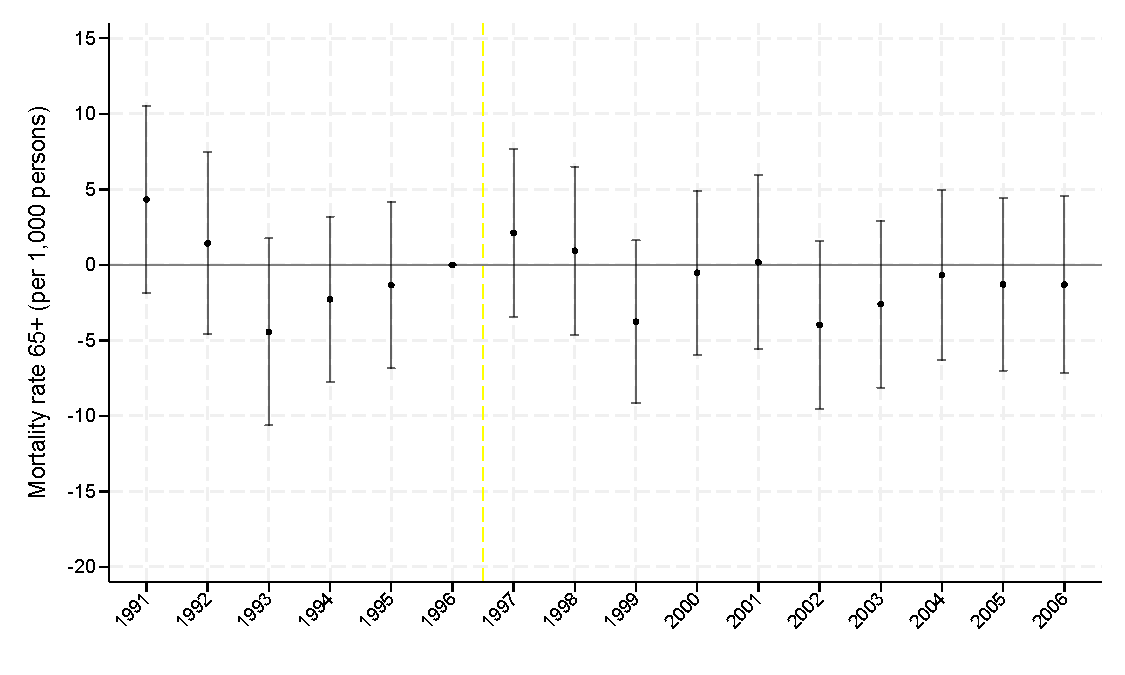
\includegraphics[width=\textwidth, height=0.42\textheight, keepaspectratio]{Figure_2_pooled.pdf}\\
    {\scriptsize Pre-trend joint test: $F=1.81$ ($p=0.108$)}\\[4pt]
    \raggedright
    {\footnotesize
    $\begin{aligned}
    \text{MR}_{m,t} = {} & \textstyle\sum_{k \neq 1996} \beta_{k}\,\mathbf{1}[t=k] \times \textit{Int}_{m,1999} \\
    & + \textstyle\sum_{k \neq 1996} \theta_{k}\,\mathbf{1}[t=k] \times \textit{Int}_{m,2005} + \delta_{m} + \gamma_{t} + \chi_{m,t} + \varepsilon_{m,t}
    \end{aligned}$}\\[3pt]
    {\scriptsize \textbf{Identification:} conditional on FEs and $\textit{Intensity}_{2005}$, municipalities with higher $\textit{Intensity}_{1999}$ would have followed parallel mortality trends absent the program}
  \end{column}
  \begin{column}{0.44\textwidth}
    \centering {\small (b) Females}\\
    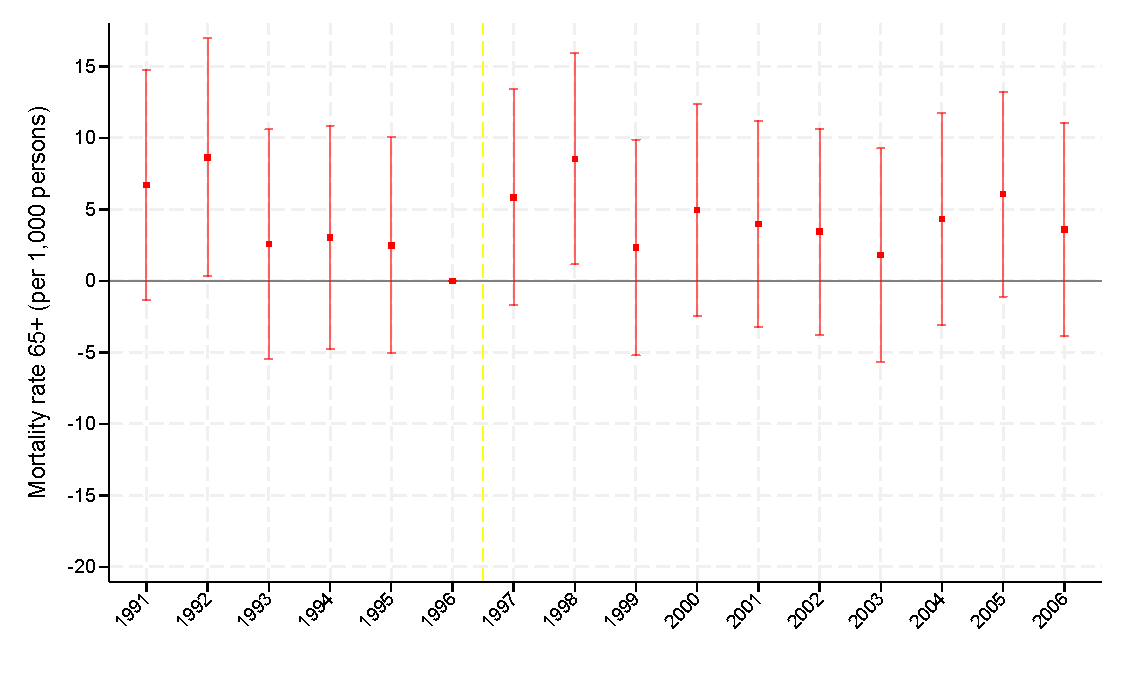
\includegraphics[width=\textwidth, height=0.30\textheight, keepaspectratio]{Figure_2_female.pdf}\\
    {\scriptsize Pre-trend joint test: $F=1.08$ ($p=0.370$)}\\[2pt]
    {\small (c) Males}\\
    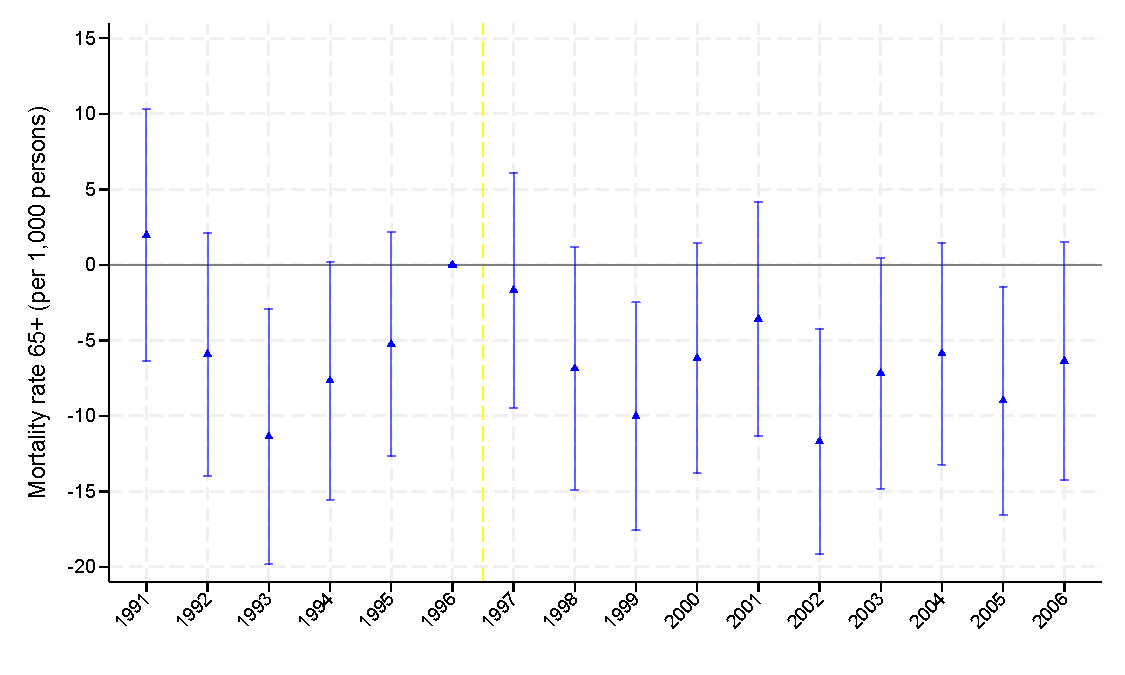
\includegraphics[width=\textwidth, height=0.30\textheight, keepaspectratio]{Figure_2_male.pdf}\\
    {\scriptsize Pre-trend joint test: $F=2.63$ (\textcolor{redUT}{$p=0.023$})}
  \end{column}
\end{columns}
\end{frame}

\note{The event study estimates one coefficient per year, relative to 1996, the last pre-program year, with the same controls and weights as the main specification. Identification requires that, conditional on fixed effects and later-phase intensity, municipalities with higher early intensity would have followed parallel mortality trends without the program; restricting to highly marginalized municipalities helps, since all were targeted and they differ in the speed of enrollment. The joint F-tests check the 1991-1995 coefficients. The event study shows the year-by-year coefficients. In the pooled sample, pre-program coefficients alternate in sign rather than drift, and we cannot reject that they are jointly zero; after 1997 the coefficients fluctuate around zero with no persistent decline. For females, there is no differential trend before or after the program. For males, we reject parallel pre-trends, with a p-value of 0.023: the coefficients from 1992 to 1995 are already at the same negative level as after 1997, so 1996 is the unusual year and there is no break at program start. We therefore do not read the male estimates as a credible program effect.}

\begin{frame}{Main Results: Effect on Elderly Mortality Rate}\label{main_results}
\vspace{-2pt}
\begin{center}
\footnotesize
\begin{tabular}{lccc}
\toprule\toprule
 & Pooled & Females & Males \\
 & (1) & (2) & (3) \\
\midrule
\textit{Intensity 1999 $\times$ post} & $-0.719$ & $0.620$ & $-2.206$ \\
 & $(1.464)$ & $(1.824)$ & $(1.735)$ \\[4pt]
\quad + SES (marginality index) trend & $0.835$ & $2.516$ & $-1.037$ \\
 & $(1.487)$ & $(1.836)$ & $(1.773)$ \\
\midrule
Mean dep.\ var.\ (1991--1996) & $46.47$ & $46.11$ & $47.26$ \\
Minimum detectable effect (80\% power) & $4.10$ & $5.11$ & $4.86$ \\
Pre-trend joint test, $p$-value & $0.108$ & $0.370$ & $0.023$ \\
Observations (1,119 municipalities) & $17{,}904$ & $17{,}904$ & $17{,}904$ \\
\midrule
$\textit{Intensity}_{2005} \times$ post control & Y & Y & Y \\
Seguro Popular & Y & Y & Y \\
Weights & Y & Y & Y \\
Mean Intensity 1999 (\%) & $44.4$ & $44.4$ & $44.4$ \\
\bottomrule\bottomrule
\end{tabular}

\vspace{2pt}
{\scriptsize MDE $= (1.96 + 0.84) \times$ SE (80\% power, 5\% level); pooled: $2.80 \times 1.464 = 4.10$ vs.\ BR's $-6.37$.}
\end{center}
\end{frame}

\note{Across all three columns, the effect of early-phase Progresa intensity on elderly mortality is small and statistically insignificant, with or without a socioeconomic trend. We do not report the 2005 intensity coefficient: it is a control with no stand-alone interpretation. Importantly, this is not a power artifact: at 80 percent power, the pooled specification can detect effects as small as 4.1 deaths per 1,000, well below the 6.4 originally reported by Barham and Rowberry. Remember that the male estimate fails the pre-trend test, so we do not put weight on it.}

%%%%%%%%%%%%%%%%%%%%%%%%%%%%%%%%%%%%%%%%
%%% ROBUSTNESS %%%
%%%%%%%%%%%%%%%%%%%%%%%%%%%%%%%%%%%%%%%%
\section{Robustness}

\begin{frame}{Robustness: Functional Form and Specification}\label{robustness_ff}
\small
\begin{itemize}
  \item[$\circ$] Main result (levels) is robust across alternative functional forms:
    \vspace{4pt}
    \begin{enumerate}
      \item \textbf{Log mortality rate} --- similar coefficients, avoids large-municipality dominance
      \vspace{4pt}
      \item \textbf{Poisson with raw death counts} --- handles zero-mortality municipality-year cells; addresses \smallcite{ChenRoth2024QJE} concerns about log with zeros
      \vspace{4pt}
      \item \textbf{Age-Adjusted Mortality Rate (AAMR)} --- directly standardizes for municipal age structure
    \end{enumerate}
  \vspace{8pt}
  \item[$\circ$] All specifications: estimates remain \textbf{small and statistically insignificant}
  \vspace{8pt}
  \item[$\circ$] Event study patterns qualitatively similar across functional forms
  \vspace{8pt}
  \item[$\circ$] Also unchanged without weights, with alternative SES trend interactions, and when later-phase intensity is measured in 2004 or 2006 instead of 2005
\end{itemize}
\end{frame}

\note{We checked whether our null finding depends on how we define the outcome or the specification. Unweighted, log mortality rates, Poisson regression with raw death counts, or age-adjusted mortality rates: the result is the same, small and insignificant effects. Results also don't change with different socioeconomic trends or if we measure later-phase coverage in 2004 or 2006.}

\begin{frame}{Replicating Barham \& Rowberry (2013)}\label{br_replication}
\footnotesize

\textbf{Original BR design:} mortality regressed on a time-varying two-year lagged enrollment intensity
\begin{equation*}
\text{MR}_{m,t} = \alpha_0 + \alpha_1\,\textit{Intensity}_{m,t-2} + \delta_m + \gamma_t + \chi_{m,t} + \varepsilon_{m,t}
\end{equation*}

\textbf{Sensitivity of BR's estimate:}
\begin{itemize}
  \item[\textbf{(A)}] BR original: $-6.37$ deaths/1,000 ($p<0.01$)
  \item[\textbf{(B)}] Our close replication: $-7.06$ deaths/1,000 ($p<0.01$)
  \item[\textbf{(C)}] Add \textit{population weights}: attenuates $\approx$\textbf{47\%} to $-3.74$ deaths/1,000 ($p<0.01$)
\end{itemize}

\vspace{6pt}
\textbf{Why does weighting matter?}
\begin{itemize}
  \item[$\circ$] \textbf{Weighting:} \textit{Progresa} targeted the most isolated, smallest, and poorest communities first; these have the highest intensity \textit{and} the most volatile mortality rates, so the unweighted estimate gives them excess influence. Weighting by the elderly population makes each municipality count in proportion to its contribution to total deaths
  \vspace{4pt}
  \item[$\circ$] \textbf{By size tercile} (BR specification, weighted): the effect is concentrated in the \textbf{smallest} municipalities, $-7.34^{***}$ (mean of 154 people aged 65+), and shrinks to $-2.37$ in the middle tercile and an insignificant $-1.39$ in the largest (mean of 2,144 people aged 65+)
\end{itemize}
\end{frame}

\note{BR's original estimate is -6.37 deaths per 1,000, and we replicate it closely at -7.06. When we add population weights, the estimate drops by nearly half to -3.74, still statistically significant but substantially smaller. Splitting by municipality size shows why weights matter: the effect is concentrated in the smallest tercile, municipalities with about 150 people aged 65 and over, and it is small and insignificant in the largest. So the short-run effect becomes much smaller and depends on specification.}

\begin{frame}{Adapting the BR Design to Our Framework}\label{br_adapt}
\footnotesize

\textbf{Our adapted design:} replaces time-varying lagged intensity with fixed early-phase intensity $\times$ post indicator
\begin{equation*}
\text{MR}_{m,t} = \beta_0\,\textit{Post}_t \times \textit{Intensity}_{m,1999} + \delta_m + \gamma_t + \varepsilon_{m,t}
\end{equation*}

\vspace{-2pt}
\begin{itemize}
  \item[$\circ$] \textbf{Advantages:} common 1997 break (no forbidden comparisons) and a pre-trends test (BR's design did not allow this)
  \item[$\circ$] \textbf{BR sample, unweighted:} $-3.97$ deaths/1,000 ($p<0.01$)
  \item[$\circ$] \textbf{BR sample, with population weights:} $-1.66$ deaths/1,000 ($p<0.05$) $\to$ attenuates $\approx$58\%
  \item[$\circ$] \textbf{Highly marginalized sample, weighted:} $-1.56$ (SE 1.26) $\to$ similar point estimate, less precise
  \vspace{1pt}
  \item[$\circ$] \textbf{Magnitudes:} BR's $-6.37$ $\approx$ 1 year of life expectancy at 65; weighted $-1.66$ $\approx$ \textbf{0.24 years} at mean intensity
  \vspace{1pt}
  \item[$\circ$] \textbf{Event study:} no clean post-1997 break; males show pre-trends in both samples (next slide)
  \vspace{1pt}
  \item[$\circ$] \textbf{Conclusion:} short-run effect is about a quarter of BR's estimate, depends on weighting and sample, and is not corroborated by the event study
\end{itemize}

\end{frame}

\note{When we apply our pre/post framework to the BR sample, we can run the event study their design couldn't. The unweighted estimate is about -4, and with population weights it falls to -1.66, significant at 5 percent but 58 percent smaller. In the highly marginalized sample the weighted point estimate is similar, -1.56, but less precise. So this is mostly attenuation, plus a loss of precision. In life expectancy terms, BR's estimate is about one year at age 65; the weighted estimate is about a quarter of a year at mean intensity. And the event study, on the next slide, does not show a clean break in 1997.}

\begin{frame}{Event Study by Sex and Sample, 1992--2002}\label{fig_a6}
\vskip 2mm
\begin{figure}
  \centering
  \begin{columns}
    \begin{column}{0.5\textwidth}
      \centering {\small (a) BR Sample --- Females}\\
      \vspace{2pt}
      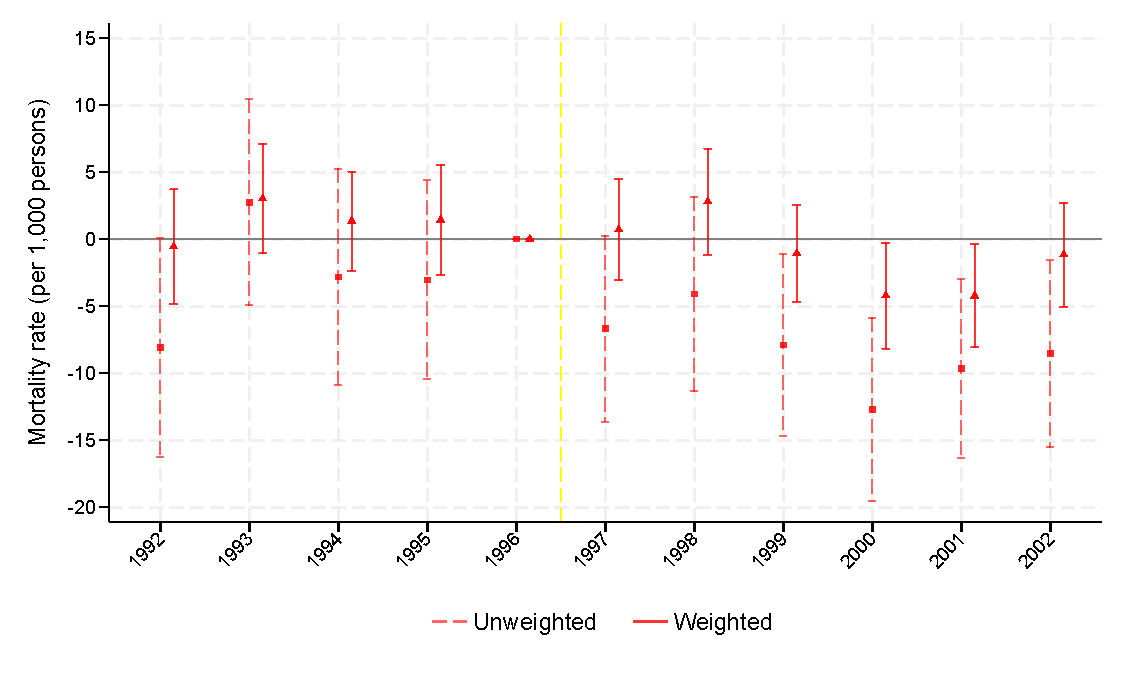
\includegraphics[width=\textwidth, height=0.38\textheight, keepaspectratio]{appendix/AF9a_emr65f_BR.pdf}
    \end{column}
    \begin{column}{0.5\textwidth}
      \centering {\small (b) High Marginalization --- Females}\\
      \vspace{2pt}
      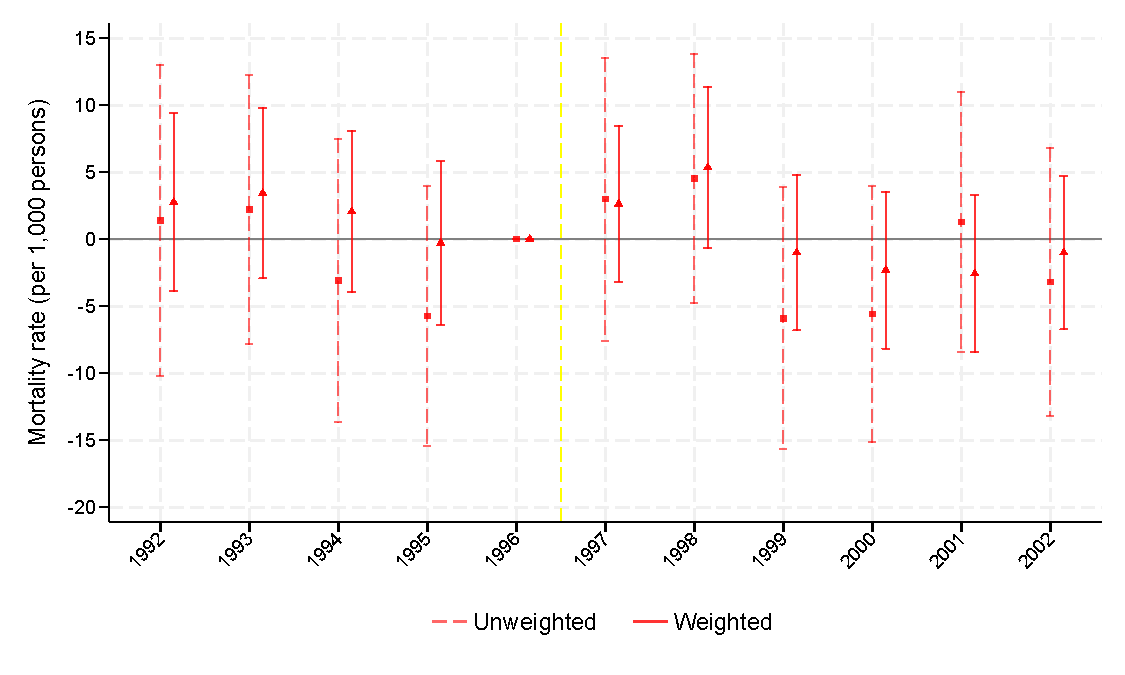
\includegraphics[width=\textwidth, height=0.38\textheight, keepaspectratio]{appendix/AF9b_emr65f_HighMarg.pdf}
    \end{column}
  \end{columns}
  \begin{columns}
    \begin{column}{0.5\textwidth}
      \centering {\small (c) BR Sample --- Males}\\
      \vspace{2pt}
      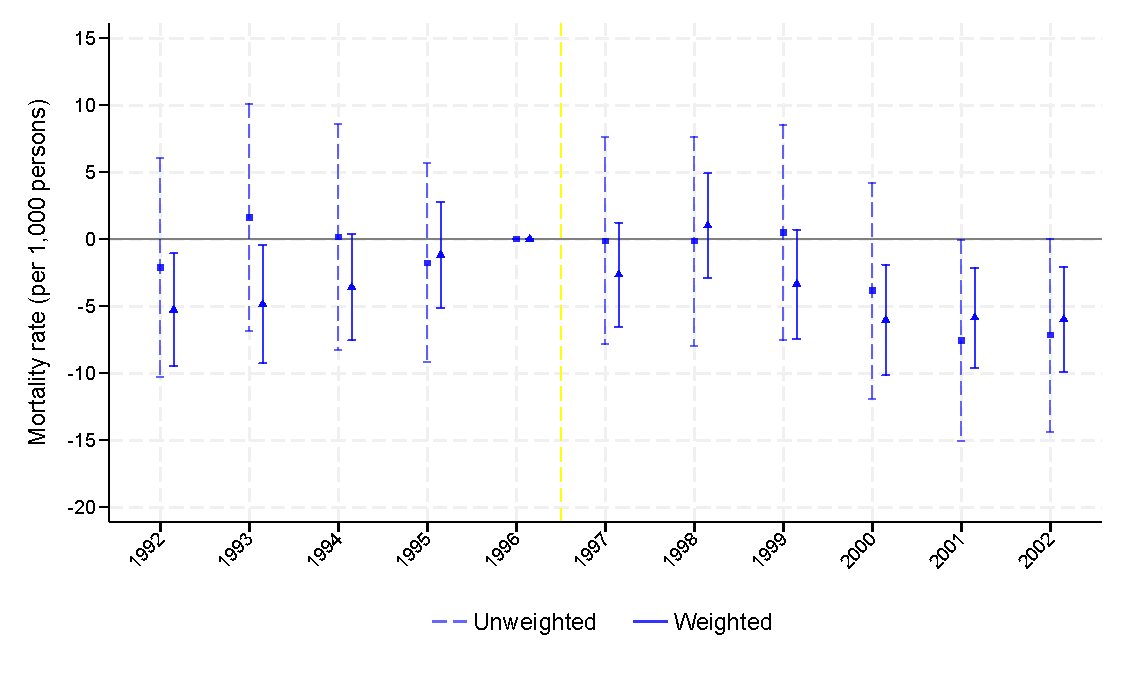
\includegraphics[width=\textwidth, height=0.38\textheight, keepaspectratio]{appendix/AF9c_emr65m_BR.pdf}
    \end{column}
    \begin{column}{0.5\textwidth}
      \centering {\small (d) High Marginalization --- Males}\\
      \vspace{2pt}
      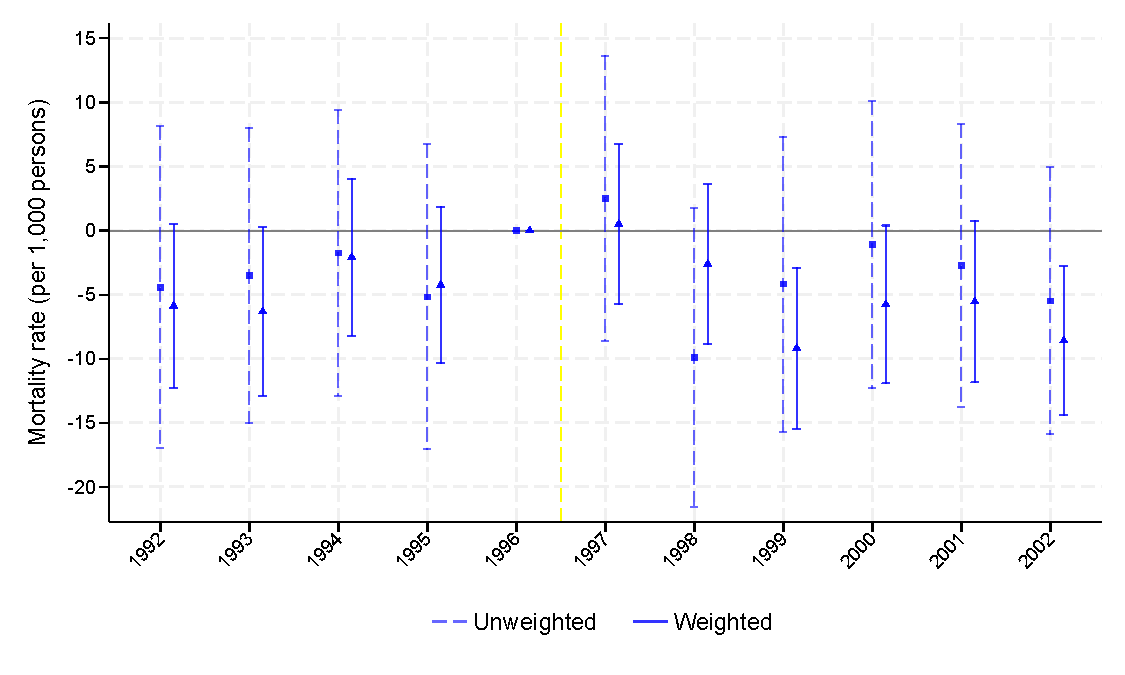
\includegraphics[width=\textwidth, height=0.38\textheight, keepaspectratio]{appendix/AF9d_emr65m_HighMarg.pdf}
    \end{column}
  \end{columns}
\end{figure}
\end{frame}

\note{This figure shows the adapted event study over 1992 to 2002, for the BR sample on the left and our highly marginalized sample on the right. For females in the BR sample, pre-trends are less pronounced, but post-program coefficients do not break from the pre-period level and overlap with it. For males, the weighted results show clear differential pre-trends in both samples. In the highly marginalized sample, neither sex shows post-program coefficients distinguishable from pre-period variation. So the short-run table estimate is not corroborated by a clean post-1997 break.}

%%%%%%%%%%%%%%%%%%%%%%%%%%%%%%%%%%%%%%%%
%%% MECHANISMS %%%
%%%%%%%%%%%%%%%%%%%%%%%%%%%%%%%%%%%%%%%%
\section{Mechanisms}

\begin{frame}{Mechanisms: Experimental Evidence (1997--1999)}\label{mechanisms_lab}
\vspace{2pt}
{\footnotesize \textbf{Data:} \textit{Progresa} evaluation (ENCASEH 1997; ENCEL 1998--1999); elderly $65+$ in eligible households, 506 treatment vs.\ 320 control localities (randomized). Municipality FE; SE clustered by locality.}
\vspace{4pt}
\begin{columns}[T]
  \begin{column}{0.62\textwidth}
    \centering
    \scriptsize
    \resizebox{\linewidth}{!}{%
    \begin{tabular}{lccccc}
    \toprule\toprule
     & \textit{Labor} & \multicolumn{3}{c}{\textit{Living arrangements}} & \textit{Health} \\
     \cmidrule(lr){2-2}\cmidrule(lr){3-5}\cmidrule(lr){6-6}
     & Weekly & Live & Live with & Only & Visits \\
     & hours & alone & children & elderly & \\
     & (1) & (2) & (3) & (4) & (5) \\
    \midrule
    \textit{Treat $\times$ 1998} & $-0.657$ & $0.006$ & $-0.003$ & $-0.007$ & \\
     & $(1.192)$ & $(0.006)$ & $(0.009)$ & $(0.007)$ & \\[3pt]
    \textit{Treat $\times$ 1999} & $0.122$ & $0.007$ & $0.027^{*}$ & $0.006$ & $-0.023$ \\
     & $(1.092)$ & $(0.009)$ & $(0.016)$ & $(0.013)$ & $(0.043)$ \\[3pt]
    \midrule
    Control mean (1997) & $14.05$ & $0.046$ & $0.693$ & $0.151$ & \\
    Control mean (1999) & & & & & $0.096$ \\
    Observations & $6{,}518$ & $7{,}025$ & $7{,}025$ & $7{,}025$ & $4{,}700$ \\
    \bottomrule\bottomrule
    \end{tabular}}
  \end{column}
  \begin{column}{0.36\textwidth}
    \scriptsize
    \begin{itemize}
      \item[$\circ$] \textbf{Labor supply:} no change in weekly hours
      \vspace{1pt}
      \item[$\circ$] \textbf{Living arrangements:} limited changes; men $+4$ pp more likely to live with children in 1999 ($p<0.05$)
      \vspace{1pt}
      \item[$\circ$] \textbf{Health visits:} no increase (no baseline; 4-week recall may miss an annual check-up)
      \vspace{1pt}
      \item[$\circ$] \textbf{Older-adults-only households} (food transfer only): no change in hours or visits
      \vspace{1pt}
      \item[$\circ$] \textbf{ENIGH 1992--2006:} income, food and health spending: imprecise nulls (limited power)
    \end{itemize}
  \end{column}
\end{columns}
\end{frame}

\note{Using the randomized evaluation data, we test whether Progresa changed the behavior of older adults in eligible households. Hours worked did not change. Living arrangements barely changed; the one exception is that older men were about 4 percentage points more likely to live with children in 1999. We find no increase in health visits, although this measure has no baseline and a four-week recall, so it may miss an annual check-up and does not contradict earlier evidence of higher utilization. In households made up only of older adults, which receive only the food transfer, hours and visits did not change either. In the ENIGH, effects on labor income, food spending and health spending are imprecise and insignificant, so we cannot rule out small effects.}

%%%%%%%%%%%%%%%%%%%%%%%%%%%%%%%%%%%%%%%%
%%% CONCLUSION %%%
%%%%%%%%%%%%%%%%%%%%%%%%%%%%%%%%%%%%%%%%
\section{Conclusion}

\begin{frame}{Concluding Remarks}\label{conclusion}
\footnotesize
\begin{itemize}
  \item[$\circ$] \textbf{Main finding:} \textit{earlier} exposure to \textit{Progresa} produced \textbf{no detectable reduction} in mortality of adults $65+$ (1997--2006)
    \begin{itemize}
      \item Robust to weighting, functional form, SES trends, Seguro Popular; male estimates fail the pre-trend test
      \item Informative null: detects effects $\geq 4.1$ deaths/1,000 (BR: $-6.37$); estimand is earlier vs.\ later exposure
    \end{itemize}
  \vspace{1pt}
  \item[$\circ$] \textbf{Short-run evidence revisited:} the \smallcite{BarhamRowberry2013JDE} estimate becomes  smaller
    \begin{itemize}
      \item Weighting attenuates it by $\approx 50\%$; concentrated in the smallest municipalities; no clean 1997 break
      \item Weighted estimate implies $\approx$0.24 years of life expectancy at 65 (vs.\ $\approx$1 year)
    \end{itemize}
  \vspace{1pt}
  \item[$\circ$] \textbf{Mechanisms:} no effects on labor supply or health visits; limited changes in living arrangements; income and nutrition imprecise
  \vspace{1pt}
  \item[$\circ$] \textbf{Interpretation:} gains in utilization and hypertension diagnosis \smallcite{BehrmanParker2013Demography, aguila2024conditional} did not translate into detectable survival gains
    \begin{itemize}
      \item Child-labeled transfers paid to mothers reach the elderly only indirectly; pensions paid \textit{directly} to older adults reduce mortality \smallcite{Menares2026JHR, MiglinoNavarrete2023AEJP}
    \end{itemize}
\end{itemize}
\end{frame}

\note{To summarize: earlier exposure to Progresa did not detectably reduce older-adult mortality over its first ten years, and our design had the power to detect effects of the size previously reported. Remember this compares earlier with later exposure. The earlier short-run estimate becomes much smaller once we weight by population and is concentrated in tiny municipalities. In the experimental data, labor supply and health visits did not change, and living arrangements changed little. This does not mean Progresa had no benefits for older adults: it improved utilization and hypertension diagnosis, but those improvements did not translate into survival gains we can detect. Programs that pay older adults directly, like pensions, have shown mortality effects.}

\begin{frame}[noframenumbering, plain]
\begin{center}
\Huge{\color{Blue}Thank you!} \\[12pt]
\small{
  Felipe Menares \\
  \texttt{felipeme@iadb.org} \\[8pt]
  \textcolor{gray}{All data publicly available from INEGI}
}
\end{center}
\end{frame}

%%%%%%%%%%%%%%%%%%%%%%%%%%%%%%%%%%%%%%%%
%%% BACKUP %%%
%%%%%%%%%%%%%%%%%%%%%%%%%%%%%%%%%%%%%%%%
\appendix
\backupbegin
\section*{Backup}

\begin{frame}{Backup: Cause-of-Death Analysis}\label{cod}
\vspace{2pt}
\begin{center}
\scriptsize
\resizebox{\textwidth}{!}{%
\begin{tabular}{lccccccccc}
\toprule\toprule
 & Cancer & Diabetes & Ill-defined & Respiratory & Cardiovascular & Infectious & Nutritional & Accidents & Other \\
 & (1) & (2) & (3) & (4) & (5) & (6) & (7) & (8) & (9) \\
\midrule
\textit{Intensity 1999 $\times$ post} & $-0.887^{***}$ & $-0.508^{**}$ & $-0.574^{***}$ & $-0.313$ & $1.530^{*}$ & $0.619$ & $-0.102$ & $0.102$ & $-0.591$ \\
 & $(0.266)$ & $(0.247)$ & $(0.221)$ & $(0.439)$ & $(0.822)$ & $(0.392)$ & $(0.488)$ & $(0.078)$ & $(0.911)$ \\
Romano--Wolf $p$-value & $[0.008]$ & $[0.282]$ & $[0.077]$ & $[1.000]$ & $[0.377]$ & $[0.574]$ & $[1.000]$ & $[0.777]$ & $[1.000]$ \\
Mean (1991--1996) & $1.70$ & $1.63$ & $1.00$ & $4.34$ & $14.01$ & $3.68$ & $4.35$ & $0.21$ & $15.54$ \\
\bottomrule\bottomrule
\end{tabular}}
\end{center}
\vspace{4pt}
\small
\begin{itemize}
  \item[$\circ$] Pooled sample; nine causes following \cite{BarhamRowberry2013JDE}'s classification
  \item[$\circ$] After Romano--Wolf correction, only \textbf{cancer} survives --- a cause BR treat as unlikely to be affected by \textit{Progresa} $\to$ read as residual differential trends, not a program effect
  \item[$\circ$] Ill-defined causes likely reflect changes in cause-of-death coding; no visual break at 1997 in cause-specific event studies
\end{itemize}
\end{frame}

\note{We also looked at cause-specific mortality. Before correcting for multiple testing, cancer, ill-defined causes, and diabetes go down, and cardiovascular goes up. After the Romano-Wolf correction for nine hypotheses, only cancer survives, and there is no plausible mechanism by which Progresa would reduce cancer mortality over this horizon, so we read it as residual trends. The ill-defined result may reflect better death certificate coding.}

\begin{frame}{Backup: Migration of Older Adults}\label{migration}
\vspace{2pt}
\begin{center}
\small
\begin{tabular}{lccc}
\toprule\toprule
 & \multicolumn{2}{c}{Log population 65+} & Log pop.\ 65+ relative \\
 & All years & Census years & to ages 50--64 (DDD) \\
 & (1) & (2) & (3) \\
\midrule
Pooled & $0.167^{***}$ & $0.207^{***}$ & $-0.034$ \\
 & $(0.023)$ & $(0.028)$ & $(0.031)$ \\[3pt]
Females & $0.180^{***}$ & $0.223^{***}$ & $-0.046$ \\
 & $(0.024)$ & $(0.029)$ & $(0.035)$ \\[3pt]
Males & $0.158^{***}$ & $0.196^{***}$ & $0.001$ \\
 & $(0.025)$ & $(0.030)$ & $(0.039)$ \\
\bottomrule\bottomrule
\end{tabular}
\end{center}
\vspace{2pt}
\footnotesize
\begin{itemize}
  \item[$\circ$] Population 65+ grows faster in high-intensity municipalities, but so does the population 50--64
  \item[$\circ$] Triple difference (municipality$\times$year, municipality$\times$age, year$\times$age FE): \textbf{no differential change for the 65+} $\to$ no evidence of selective elderly migration
  \item[$\circ$] Census-year event studies: pre-program coefficient not significant ($p=0.18$ pooled, log)
\end{itemize}
\end{frame}

\note{A natural concern is that Progresa changed who lives in these municipalities. The population aged 65 and over does grow faster in high-intensity municipalities, but so does the population aged 50 to 64. Once we compare the two age groups in a triple difference, there is no differential change for older adults. This is consistent with Stecklov and coauthors, who find no effects of Progresa on migration of older household members.}

\begin{frame}{Backup: Without the Later-Phase Control; By Municipality Size}\label{nocontrol_size}
\small
\textbf{(a) Main specification without $\textit{Intensity}_{2005} \times$ post}
\begin{center}
\begin{tabular}{lccc}
\toprule
 & Pooled & Females & Males \\
\midrule
\textit{Intensity 1999 $\times$ post} & $-2.255^{*}$ & $-2.466$ & $-2.095$ \\
 & $(1.276)$ & $(1.534)$ & $(1.469)$ \\
\bottomrule
\end{tabular}
\end{center}
\vspace{4pt}
\textbf{(b) BR sample by size tercile (1992--2002), weighted}
\begin{center}
\begin{tabular}{lcccc}
\toprule
 & All & Small & Medium & Large \\
\midrule
Adapted design ($\textit{Intensity}_{1999} \times$ post) & $-1.660^{**}$ & $-2.908$ & $-1.317$ & $-0.029$ \\
 & $(0.807)$ & $(2.483)$ & $(1.359)$ & $(1.193)$ \\
BR two-year lagged intensity & $-3.740^{***}$ & $-7.343^{***}$ & $-2.372$ & $-1.393$ \\
 & $(0.786)$ & $(2.088)$ & $(1.450)$ & $(1.218)$ \\
Mean population 65+ & 951 & 154 & 556 & 2,144 \\
\bottomrule
\end{tabular}
\end{center}
\end{frame}

\note{Without the later-phase control, the pooled estimate is -2.3, significant only at 10 percent; this specification conflates the timing of exposure with overall program intensity. By size tercile in the BR sample, both the adapted design and BR's specification produce their largest effects in the smallest municipalities, with mean populations of about 150 older adults, and essentially zero in the largest ones.}

\backupend

{\tiny\bibliography{bibliography}}

\end{document}
